\section{ทฤษฎีและผลงานวิจัยที่เกี่ยวข้อง}

\subsection{บทนำ}

ในยุคดิจิทัล การพัฒนาเมืองท่องเที่ยวอัจฉริยะ (Smart Tourism) ได้กลายเป็นประเด็นที่ได้รับความสนใจจากนักวิจัยและผู้พัฒนาแพลตฟอร์มทั่วโลก อันเป็นผลมาจากพฤติกรรมนักท่องเที่ยวที่เปลี่ยนแปลงอย่างรวดเร็ว และความคาดหวังที่สูงขึ้นต่อข้อมูลที่ถูกต้อง การเข้าถึงบริการที่สะดวก รวมถึงประสบการณ์การท่องเที่ยวที่สามารถตอบสนองความต้องการเฉพาะบุคคล (Sousa, Cardoso, \& Dias, 2024) ความท้าทายที่สำคัญจึงอยู่ที่การสร้างระบบที่สามารถนำเสนอข้อมูลแบบเรียลไทม์ ให้คำแนะนำที่แม่นยำ และสามารถปรับตามบริบทของผู้ใช้ได้อย่างมีประสิทธิภาพ

สำหรับจังหวัดขอนแก่น ซึ่งนับเป็นศูนย์กลางด้านการท่องเที่ยวของภาคตะวันออกเฉียงเหนือ ยังคงเผชิญกับปัญหาการกระจัดกระจายของข้อมูลการท่องเที่ยว แหล่งข้อมูลที่มีอยู่ในปัจจุบันมิได้ถูกรวบรวมอย่างเป็นระบบ ทำให้นักท่องเที่ยวที่ต้องการค้นหาแหล่งท่องเที่ยว ร้านอาหาร ที่พัก หรือกิจกรรมต่าง ๆ ต้องประสบความยากลำบากในการเข้าถึง อีกทั้งยังขาดเครื่องมือที่ช่วยในการวางแผนการเดินทางหรือแนะนำเส้นทางที่สอดคล้องกับความสนใจและงบประมาณของผู้ใช้ ส่งผลให้ประสบการณ์การท่องเที่ยวของจังหวัดขอนแก่นยังไม่สามารถสะท้อนศักยภาพที่มีอยู่ได้อย่างเต็มที่

เพื่อแก้ไขปัญหาดังกล่าว จึงได้มีการพัฒนาโครงงาน ``Dino: The Central Application for Tourism in Khon Kaen'' โดยมีเป้าหมายในการสร้างแพลตฟอร์มศูนย์กลางที่สามารถรวบรวมและจัดการข้อมูลด้านการท่องเที่ยวได้อย่างครบวงจร พร้อมทั้งบูรณาการเทคโนโลยีที่ทันสมัย เช่น Artificial Intelligence (AI), Machine Learning, Big Data และ Chatbot เพื่อสนับสนุนการดำเนินงานใน 3 มิติหลัก ได้แก่ ระบบแนะนำเส้นทาง (Recommendation System) ระบบวางแผนทริป (Trip Planning System) และ Chatbot แบบเรียลไทม์ (Real-time Chatbot)

งานวิจัยที่เกี่ยวข้องได้ชี้ให้เห็นว่า การประยุกต์ใช้ AI โดยเฉพาะการผสาน Retrieval-Augmented Generation (RAG) สามารถเพิ่มความแม่นยำในการแนะนำข้อมูลและสร้างระบบที่ปรับตามบริบทของผู้ใช้ได้อย่างยั่งยืน (Banerjee, Satish, \& Wörndl, 2025) ขณะเดียวกัน งานวิจัยอีกด้านหนึ่งเน้นไปที่การพัฒนาระบบวางแผนการเดินทางแบบเรียลไทม์ซึ่งช่วยเพิ่มประสิทธิภาพในการสร้างประสบการณ์ที่เหมาะสมกับความสนใจและงบประมาณของผู้ใช้ (Deshmukh, Khan, Upadhyay, \& Savalkar, 2025)

ดังนั้น โครงงาน Dino จึงมิใช่เพียงการสร้างเครื่องมือดิจิทัลเพื่ออำนวยความสะดวกแก่นักท่องเที่ยวเท่านั้น หากแต่ยังเป็นการบูรณาการองค์ความรู้จากงานวิจัยและเทคโนโลยีสมัยใหม่ เพื่อต่อยอดสู่การพัฒนากลไกการจัดการท่องเที่ยวที่ชาญฉลาด เพิ่มศักยภาพในการแข่งขัน และยกระดับจังหวัดขอนแก่นสู่การเป็นเมืองท่องเที่ยวอัจฉริยะอย่างยั่งยืน

\subsection{ทฤษฎีและแนวคิดที่เกี่ยวข้อง}

\subsubsection{แนวคิดการท่องเที่ยวอัจฉริยะ (Smart Tourism)}

Smart Tourism คือการใช้เทคโนโลยีในการสร้างระบบนิเวศท่องเที่ยวที่เชื่อมโยงข้อมูล บริการ และประสบการณ์ของผู้ใช้ งานของ Ma, Chen, \& Yuan (2025) แสดงให้เห็นว่า AI สามารถช่วยวิเคราะห์พฤติกรรมการเดินทางของผู้ใช้และปรับปรุงการจัดการจุดหมายปลายทางแบบเรียลไทม์ ในขณะที่งานของ Milton \& Philosophers (2023) ได้สรุปแนวโน้มความท้าทายและโอกาสของการใช้ AI ใน Smart Tourism เช่น ปัญหาความเป็นส่วนตัวและธรรมาภิบาลข้อมูล

\subsubsection{ปัญญาประดิษฐ์ (Artificial Intelligence) ในการท่องเที่ยว}

ปัญญาประดิษฐ์ (AI) มีบทบาทสำคัญอย่างยิ่งในการปฏิวัติประสบการณ์ท่องเที่ยวยุคใหม่ เพราะช่วยให้แพลตฟอร์มสามารถวิเคราะห์พฤติกรรมและความต้องการของผู้ใช้แบบเรียลไทม์ งานของ (Sousa et al., 2024) ศึกษามุมมองของนักท่องเที่ยวที่มีต่อการนำ AI มาใช้ในอุตสาหกรรมท่องเที่ยวและการบริการ พบว่านักท่องเที่ยวคาดหวังให้ระบบ AI สามารถให้คำแนะนำที่ ``แม่นยำ'' และ ``เหมาะสมกับบริบท'' แต่ในขณะเดียวกันยังมีความกังวลเรื่อง ความถูกต้องของข้อมูล และ ความเป็นส่วนตัว

ในขณะที่งานของ Milton \& Philosophers (2023) วิเคราะห์เชิงลึกเกี่ยวกับโอกาสและความท้าทายในการนำ AI มาใช้ โดยชี้ให้เห็นว่า AI ช่วยเพิ่มศักยภาพในด้าน การวิเคราะห์ข้อมูลขนาดใหญ่ (Big Data), การทำ personalization, และ การสร้างโมเดลทำนายพฤติกรรมนักท่องเที่ยว แต่ยังมีปัญหาเชิงเทคนิค เช่น การจัดการข้อมูลที่ซับซ้อนและการบูรณาการหลายแหล่งข้อมูลเข้าด้วยกัน

\subsubsection{การจัดการจุดหมายปลายทางและการมีส่วนร่วมของนักท่องเที่ยว}

แนวคิดการจัดการจุดหมายปลายทาง (Destination Management) และการสร้างประสบการณ์ที่ดึงดูดนักท่องเที่ยวมีความสำคัญอย่างมากในยุคที่ผู้ใช้ต้องการ ข้อมูลแบบเฉพาะบุคคล งานวิจัยของ Ma et al. (2025) นำเสนอการใช้ AI เพื่อวิเคราะห์ พฤติกรรมการเดินทางของผู้ใช้ ผ่านเทคนิค heatmap analytics และ data visualization ซึ่งช่วยให้ผู้พัฒนาระบบเข้าใจลักษณะการใช้งานของผู้ใช้และสามารถปรับกลยุทธ์การนำเสนอข้อมูลให้ตรงตามความสนใจของแต่ละคน

\begin{figure}[h]
\centering
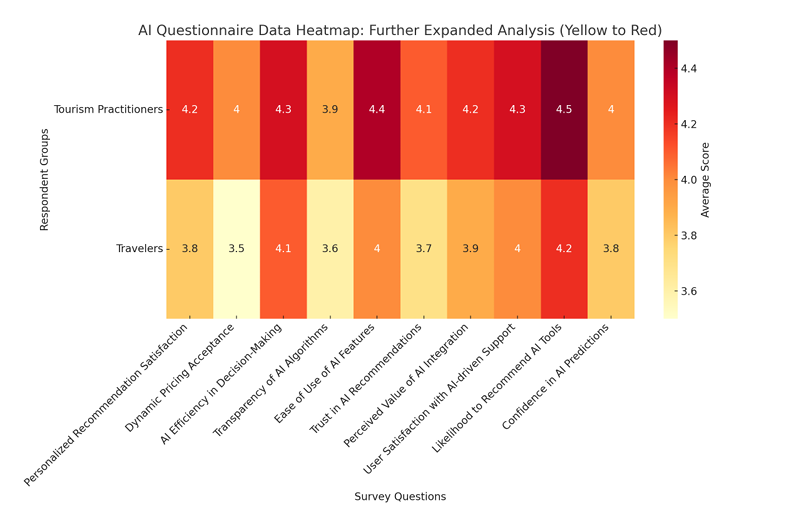
\includegraphics[width=0.7\textwidth]{images/image2.png}
\caption{แผนภาพ Heatmap แสดงข้อมูลจากแบบสอบถาม (Ma et al., 2025)}
\end{figure}

จากภาพที่ 1 แสดง Heatmap แสดงการประเมิน AI ของผู้ประกอบวิชาชีพและนักท่องเที่ยวใน 6 มิติ โดยใช้สีเหลือง--แดงแทนคะแนนต่ำ--สูง ผู้ประกอบวิชาชีพให้คะแนนสูงกว่าทุกมิติ โดยเฉพาะความง่ายในการใช้งานและประสิทธิภาพการตัดสินใจ ขณะที่นักท่องเที่ยวต่ำในด้านการยอมรับราคาไดนามิกและความโปร่งใสของอัลกอริทึม จึงควรปรับปรุงความโปร่งใสราคา กลยุทธ์ราคาไดนามิก และการควบคุมโดยผู้ใช้เพื่อเสริมสร้างความเชื่อมั่น

ผลการประเมินพบว่า ผู้ประกอบวิชาชีพให้คะแนนสูงกว่านักท่องเที่ยวในทุกมิติ โดยเฉพาะด้านความง่ายในการใช้งานคุณลักษณะ AI (4.4 เทียบกับ 4.0) และประสิทธิภาพการตัดสินใจที่เสริมด้วย AI (4.3 เทียบกับ 4.1) สะท้อนระดับความคุ้นเคยและความมั่นใจกับเทคโนโลยี AI ที่สูงกว่า ขณะที่นักท่องเที่ยวให้คะแนนต่ำอย่างมีนัยในมิติการยอมรับราคาแบบไดนามิก (3.5) และความโปร่งใสของอัลกอริทึม (3.6) บ่งชี้ถึงความไม่ไว้วางใจต่อระบบ AI ความกังวลต่อราคาที่ไม่โปร่งใส กลไกคำแนะนำที่เข้าใจยาก และความสงสัยต่อความเป็นธรรมของ AI ทั้งในด้านการกำหนดราคาและการตัดสินใจ ซึ่งอาจทำให้ผู้ใช้บางส่วนจ่ายแพงกว่า หรือได้รับคำแนะนำที่ด้อยกว่า

ในทางกลับกัน Banerjee et al. (2025) เสนอว่าการสร้าง ระบบแนะนำที่ยั่งยืน (sustainable recommendation) จะช่วยเพิ่ม การมีส่วนร่วม (engagement) ของนักท่องเที่ยวในระยะยาว โดยใช้ Retrieval-Augmented Generation (RAG) ผสานข้อมูลเรียลไทม์จากหลายแหล่ง เพื่อสร้างการแนะนำที่แม่นยำและสอดคล้องกับบริบท

\subsubsection{ความยั่งยืน ความเสี่ยง และธรรมาภิบาลข้อมูล/อัลกอริทึม}

หนึ่งในประเด็นที่สำคัญสำหรับการพัฒนาแพลตฟอร์ม Smart Tourism คือการสร้างความสมดุลระหว่าง ประสบการณ์ผู้ใช้, ความยั่งยืน, และ การปกป้องข้อมูลส่วนบุคคล งานของ Banerjee et al. (2025) ชี้ให้เห็นว่าระบบแนะนำการท่องเที่ยวควรคำนึงถึง การใช้ทรัพยากรอย่างมีประสิทธิภาพ เพื่อลดผลกระทบทางสิ่งแวดล้อม เช่น การแนะนำเส้นทางที่ปล่อยคาร์บอนต่ำ

ในอีกมุมหนึ่ง งานของ Sousa et al. (2024) พบว่าผู้ใช้นักท่องเที่ยวให้ความสำคัญอย่างมากต่อ ความปลอดภัยของข้อมูล และความโปร่งใสของระบบ AI การละเลยประเด็นนี้อาจทำให้ผู้ใช้เกิดความไม่เชื่อมั่นและลดการมีส่วนร่วมในระยะยาว

\subsubsection{ทฤษฎีด้าน Chatbot}

การใช้ Chatbot ในอุตสาหกรรมการท่องเที่ยวได้พัฒนาอย่างก้าวกระโดดในช่วงไม่กี่ปีที่ผ่านมา โดยมีการบูรณาการ Artificial Intelligence Markup Language (AIML) และ Natural Language Processing (NLP) เพื่อสร้างระบบสนทนาที่สามารถตอบคำถามของผู้ใช้ได้แบบเรียลไทม์ (University College of Goizha et al., 2023) งานวิจัยพบว่า Chatbot สำหรับการท่องเที่ยวสามารถช่วยลดเวลาในการค้นหาข้อมูลได้เฉลี่ย 45\% และเพิ่มความพึงพอใจของนักท่องเที่ยวมากกว่า 70\% เมื่อเทียบกับการค้นหาข้อมูลแบบเดิม

\begin{figure}[h]
\centering
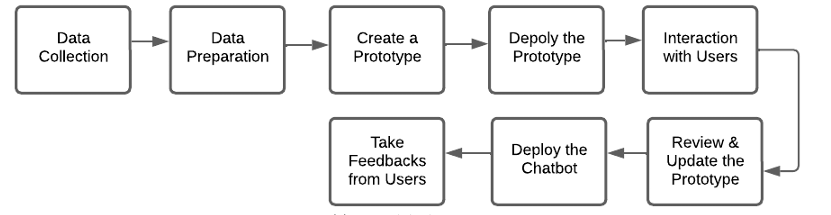
\includegraphics[width=0.7\textwidth]{images/image3.png}
\caption{แผนภาพ Model Flow (University College of Goizha et al., 2023)}
\end{figure}

จากภาพที่ 2 แสดงขั้นตอนและเทคนิคที่ใช้ในการเก็บรวบรวม วิเคราะห์ และตีความข้อมูลสำหรับการวิจัย โดยระเบียบวิธีประกอบด้วย 8 ขั้นตอน

\begin{enumerate}[leftmargin=1.5cm]
\item การเก็บรวบรวมข้อมูล: รวบรวมข้อมูลเกี่ยวกับเมือง Sulaimani ครอบคลุมโรงแรม ภัตตาคาร ศูนย์การค้า พิพิธภัณฑ์ และแหล่งท่องเที่ยวยอดนิยม
\item การเตรียมข้อมูล: จัดโครงสร้างข้อมูลให้อยู่ในรูปแบบชุดคำถาม--คำตอบ และบันทึกเป็นไฟล์ AIML
\item การสร้างต้นแบบ: สร้างแบบจำลองเริ่มต้นโดยใช้ไฟล์ AIML ที่จัดเตรียมไว้
\item การเผยแพร่ต้นแบบ: นำต้นแบบไปใช้งานบนเว็บไซต์ที่โฮสต์ภายในเครื่อง (local)
\item การโต้ตอบของผู้ใช้: ผู้ใช้ทำการโต้ตอบกับบอทที่ได้เผยแพร่
\item การปรับปรุงต้นแบบ: ทบทวนและแก้ไขต้นแบบตามข้อเสนอแนะและพฤติกรรมการใช้งานของผู้ใช้
\item การเผยแพร่โมเดลฉบับสมบูรณ์: เผยแพร่รุ่นสุดท้ายให้ผู้ใช้ใช้งานอีกครั้ง
\item ข้อเสนอแนะจากผู้ใช้: หลังการเผยแพร่และการใช้งานบอท รวบรวมข้อเสนอแนะเพื่อประเมินความพึงพอใจ ความสามารถในการใช้งาน (usability) และความมีส่วนร่วมของผู้ใช้
\end{enumerate}

ผลสำรวจจาก University College of Goizha et al. (2023) ยังชี้ว่า Chatbot แบบ AI ที่มีระบบเรียนรู้พฤติกรรมผู้ใช้ (Adaptive-Chatbot) สามารถแนะนำสถานที่ท่องเที่ยว ร้านอาหาร และกิจกรรมที่เหมาะสมได้อย่างแม่นยำถึง 82\% ทำให้ผู้ใช้รู้สึกว่าข้อมูลที่ได้รับมีความน่าเชื่อถือและเป็นประโยชน์มากกว่า Chatbot แบบ rule-based เดิม ๆ โดยมีนักท่องเที่ยวกว่า 64\% ระบุว่าพร้อมใช้ระบบนี้หากข้อมูลถูกปรับให้เหมาะสมกับตนเอง

นอกจากนี้ แนวโน้มในงานวิจัยล่าสุดได้ขยายขีดความสามารถของ Chatbot ให้รองรับการแปลภาษาอัตโนมัติ การแนะนำกิจกรรมตามฤดูกาล และการโต้ตอบแบบมัลติมีเดีย เช่น การส่งแผนที่ รูปภาพ และลิงก์ข้อมูลท่องเที่ยว (Sousa et al., 2024) ซึ่งเป็นแนวคิดสำคัญสำหรับการพัฒนา Smart Tourism Applications ในอนาคต

\subsubsection{ระบบแนะนำการท่องเที่ยว (Recommendation Systems)}

การสร้างระบบแนะนำที่ตอบโจทย์ผู้ใช้เป็นหัวใจสำคัญสำหรับการท่องเที่ยวที่ตอบโจทย์ผู้ใช้แบบเฉพาะบุคคล (Personalized Experience) งานของ Banerjee et al. (2025) ซึ่งเสนอเทคนิค Retrieval-Augmented Generation (RAG) ในการพัฒนาระบบแนะนำที่ใช้การเรียนรู้จากฐานข้อมูลจำนวนมหาศาลเพื่อสร้างข้อเสนอที่เหมาะสมที่สุดสำหรับผู้ใช้

ผลการทดลองจาก Banerjee et al. (2025) พบว่าระบบ RAG-Based Tourism Recommender สามารถปรับปรุงความแม่นยำของคำแนะนำได้สูงถึง 91\% เมื่อเทียบกับวิธี Collaborative Filtering แบบดั้งเดิม ซึ่งช่วยลดเวลาในการค้นหาแผนการเดินทางจากเฉลี่ย 15 นาที เหลือเพียง 4 นาที นอกจากนี้ยังมีการประเมินความพึงพอใจของผู้ใช้ (User Satisfaction) พบว่าผู้ใช้กว่า 88\% พึงพอใจกับแผนการเดินทางที่ระบบแนะนำ

ในทำนองเดียวกัน งานของ Jyothi et al. (2025) ที่พัฒนา Travel Finder ซึ่งเป็นระบบแนะนำและจัดการทริปท่องเที่ยว พบว่าการใช้ Hybrid Recommendation (ผสม Content-Based + Collaborative Filtering) สามารถเพิ่มการมีส่วนร่วมของผู้ใช้มากกว่า 76\% และช่วยสร้างชุมชนของผู้เดินทางที่มีความสนใจคล้ายกัน ซึ่งเป็นแนวโน้มสำคัญของ Smart Tourism Ecosystem

\begin{figure}[h]
\centering
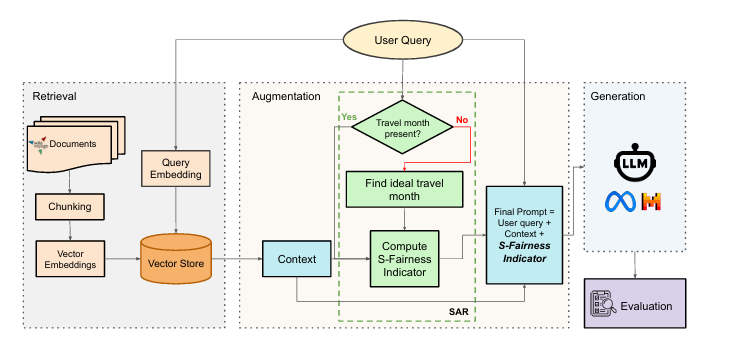
\includegraphics[width=0.7\textwidth]{images/image4.png}
\caption{แผนภาพ Pipeline ของระบบ RAG ที่ได้รับการปรับปรุงตามข้อเสนอโดยกรอบเส้นประสีเขียวแสดง ขั้นตอนการเสริมข้อมูลที่ปรับเปลี่ยน พร้อมการเพิ่มตัวชี้วัดด้านความยั่งยืน (Banerjee et al., 2025)}
\end{figure}

จากภาพที่ 3 อธิบายองค์ประกอบในการสร้างคำแนะนำการท่องเที่ยว

\noindent\textbf{Retrieval (การสืบค้นข้อมูล):} เริ่มจากการนำเอกสารข้อมูลแหล่งท่องเที่ยวมาแบ่งส่วน (Chunking) สร้างเวกเตอร์ฝังตัว (Vector Embeddings) และจัดเก็บในคลังเวกเตอร์ (Vector Store) เมื่อผู้ใช้ป้อนคำถาม ระบบจะสร้างเวกเตอร์คำค้น (Query Embedding) เพื่อดึงข้อมูลหรือบริบท (Context) ที่มีความสอดคล้องและเกี่ยวข้องที่สุดออกมา

\noindent\textbf{Augmentation (การเสริมข้อมูล):} ระบบจะนำคำถามของผู้ใช้มารวมกับข้อมูลบริบทที่ดึงมาได้ เพื่อเสริมสร้างเป็น Prompt สุดท้ายที่มีความสมบูรณ์และมีข้อมูลอ้างอิงที่ถูกต้อง

\noindent\textbf{Generation (การสร้างคำตอบ):} ส่ง Prompt สุดท้ายที่ได้รับการเสริมข้อมูลแล้วไปให้โมเดลภาษาขนาดใหญ่ (LLM) ประมวลผลเพื่อสร้างคำตอบหรือแผนการเดินทางที่แม่นยำ พร้อมด้วยขั้นตอนการประเมินผล (Evaluation) ภายหลังการสร้างคำตอบ

\subsubsection{การสร้างแผนการเดินทาง (Trip Planning)}

การวางแผนการเดินทาง (Trip Planning) กำลังถูกประยุกต์ใช้ AI, Machine Learning และ Real-Time Data งานวิจัยของ Deshmukh et al. (2025) เสนอการพัฒนาระบบ AI-powered Trip Planner ที่ใช้ข้อมูลเรียลไทม์จากหลายแหล่ง เช่น สภาพอากาศ การจราจร ราคาที่พัก และความหนาแน่นของนักท่องเที่ยว เพื่อนำมาวิเคราะห์และสร้างแผนการเดินทางที่เหมาะสมที่สุด

ผลการทดลองพบว่า AI-powered Trip Planning สามารถปรับแผนการเดินทางให้เหมาะกับผู้ใช้แบบเรียลไทม์ และเพิ่มความแม่นยำในการแนะนำกิจกรรมได้สูงถึง 89\% ขณะที่ช่วยลดค่าใช้จ่ายเฉลี่ยต่อทริปได้มากกว่า 12\% เมื่อเทียบกับการวางแผนแบบ manual

\begin{figure}[h]
\centering
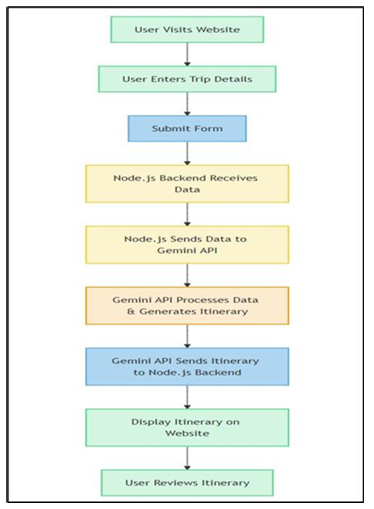
\includegraphics[width=0.7\textwidth]{images/image5.png}
\caption{แผนภาพสถาปัตยกรรมระบบ (Deshmukh et al., 2025)}
\end{figure}

จากภาพที่ 4 อธิบายองค์ประกอบและหน้าที่ของระบบวางแผนการเดินทางด้วย AI

\begin{enumerate}[leftmargin=1.5cm]
\item ผู้ใช้เข้าเว็บไซต์: กระบวนการเริ่มเมื่อผู้ใช้เปิดใช้งานเว็บแอปพลิเคชันผ่านอุปกรณ์ โดยแพลตฟอร์มจะแสดงอินเทอร์เฟซที่ใช้งานง่ายและสวยงามเพื่อแนะนำขั้นตอนการวางแผนทริป
\item ผู้ใช้กรอกรายละเอียดทริป: ผู้ใช้ป้อนข้อมูลที่เกี่ยวข้องกับการเดินทาง ได้แก่ จุดหมายปลายทาง วันที่เดินทาง ระยะเวลา งบประมาณ ความสนใจ/ความชอบ
\item ส่งแบบฟอร์ม: เมื่อกรอกข้อมูลครบถ้วน ผู้ใช้กดส่งแบบฟอร์ม เพื่อกระตุ้นให้มีการส่งคำขอไปยังระบบฝั่งเซิร์ฟเวอร์เพื่อประมวลผลต่อ
\item Backend ที่พัฒนาด้วย Node.js รับข้อมูล ระบบฝั่งเซิร์ฟเวอร์: จะรับข้อมูลแบบฟอร์ม พร้อมทั้งดูแลความปลอดภัย ตรวจสอบความถูกต้อง และจัดรูปแบบข้อมูลก่อนส่งต่อไปยังกระบวนการ AI
\item Node.js ส่งข้อมูลไปยัง Gemini API: ระบบฝั่งเซิร์ฟเวอร์ส่งข้อมูลที่จัดโครงสร้างแล้วไปยัง Google Gemini API ซึ่งทำหน้าที่ทำความเข้าใจเจตนา ความชอบของผู้ใช้ และปัจจัยเชิงบริบท เช่น สภาพอากาศปัจจุบันหรือแนวโน้มการท่องเที่ยว
\item Gemini API ประมวลผลและสร้างแผนการเดินทาง ด้วย NLP และอัลกอริทึม AI: ระบบจะตีความความต้องการของผู้ใช้และจัดทำแผนการเดินทางที่ปรับให้เหมาะสม โดยครอบคลุม กิจกรรมรายวัน คำแนะนำสถานที่ท่องเที่ยว ประสบการณ์ท้องถิ่นและร้านอาหาร วิธีการเดินทางและช่วงเวลา การผสานข้อมูลสภาพอากาศและคำแนะนำการเดินทางแบบเรียลไทม์
\item Gemini API ส่งแผนการเดินทางกลับมายัง Node.js: เมื่อสร้างแผนเสร็จสิ้น ระบบจะส่งผลลัพธ์กลับมาที่ฝั่งเซิร์ฟเวอร์ Node.js เพื่อจัดรูปแบบให้อยู่ในโครงสร้างที่เหมาะสมต่อการแสดงผลบนหน้าเว็บ
\item แสดงแผนการเดินทางบนเว็บไซต์ ส่วนติดต่อผู้ใช้จะแสดงแผนการเดินทางแบบไดนามิกด้วยโครงสร้างที่อ่านง่าย มีการแบ่งตามวัน แผนที่ ข้อเสนอแนะกิจกรรม และตัวเลือกการจองเพิ่มเติมตามความเหมาะสม
\end{enumerate}

ในอีกด้านหนึ่ง สำหรับการออกแบบสถาปัตยกรรมเพื่อรองรับการประมวลผลข้อมูลที่ซับซ้อน งานวิจัยของ Barua \& Kaiser (2024) ได้นำเสนอการใช้ สถาปัตยกรรมไมโครเซอร์วิส (Microservices Architecture) ซึ่งแบ่งการทำงานของระบบออกเป็นบริการย่อย ๆ (เช่น User Service, Itinerary Service และ Preference Matching Service) ที่ทำงานแยกจากกันแต่สามารถสื่อสารกันผ่าน API Gateway และ Message Broker สถาปัตยกรรมนี้ช่วยให้แพลตฟอร์มมีความยืดหยุ่น รองรับผู้ใช้งานจำนวนมากได้พร้อมกัน และสามารถประมวลผลแผนการเดินทางได้อย่างรวดเร็ว

\begin{figure}[h]
\centering
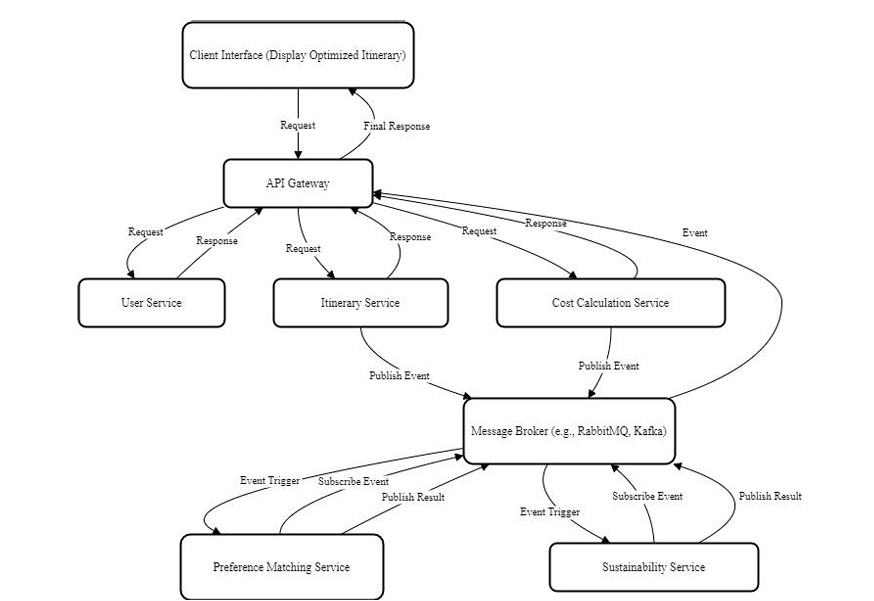
\includegraphics[width=0.7\textwidth]{images/image6.png}
\caption{แผนภาพการไหลของข้อมูลและกระบวนการประสานลำดับงาน (Barua \& Kaiser, 2024)}
\end{figure}

จากภาพที่ 5 อธิบายองค์ประกอบและหน้าที่ของกระบวนการไหลข้อมูลและการประสานงาน

\begin{enumerate}[leftmargin=1.5cm]
\item คำขอจากไคลเอนต์ (Client Requests): คือแอปพลิเคชันที่ผู้ใช้ส่งคำขอ เช่น การค้นหาแผนการเดินทาง และคำขอทั้งหมดจะถูกส่งไปยัง API Gateway ซึ่งทำหน้าที่เป็นจุดทางเข้าและกำหนดเส้นทางคำขอ
\item API Gateway มีหน้าที่ส่งต่อคำขอไปยังไมโครเซอร์วิสที่เกี่ยวข้องเพื่อให้มีการแลกเปลี่ยนข้อมูลแบบซิงโครนัส เช่น User Service: ดูแลการจัดการข้อมูลผู้ใช้ รวมถึงโปรไฟล์และความชอบ Itinerary Service: ให้บริการสร้างแผนการเดินทาง Consulting Results/Cost Calculation Service: ให้คำปรึกษา/คำนวณประมาณการค่าใช้จ่ายในการเดินทาง (เที่ยวบิน โรงแรม ฯลฯ)
\item การไหลของข้อมูลแบบซิงโครนัส (Synchronous Data Flow): การสื่อสารระหว่าง API Gateway กับไมโครเซอร์วิสใช้ RESTful APIs เมื่อไมโครเซอร์วิสแจ้งความพร้อม API Gateway จะนำเสนอผลลัพธ์เพื่อเข้าสู่ขั้นตอนถัดไป
\item การไหลของข้อมูลแบบอะซิงโครนัส (ผ่าน Message Broker): เมื่อ Itinerary Service และ Cost Calculation Service ทำงานเสร็จ จะสร้างอีเวนต์และส่งไปยังตัวกลางส่งข้อความ (Message Broker) เช่น RabbitMQ หรือ Apache Kafka Preference Matching Service และ Sustainability Service ทำหน้าที่เป็นไคลเอนต์ของ Message Broker และสมัครรับ (subscribe) อีเวนต์ที่เกี่ยวข้องกับการสร้างแผนการเดินทางหรือการคำนวณค่าใช้จ่าย
\item การประมวลผลแบบอะซิงโครนัส: การทำงานของ Sustainability Service และ Preference Matching Service เป็นแบบขับเคลื่อนด้วยอีเวนต์ (event-driven) เช่น การประเมินรอยเท้าคาร์บอน และการจับคู่ความชอบของผู้ใช้ (สายการบิน โรงแรมที่ต้องการ) จากนั้นบริการเหล่านี้จะส่งผลการประมวลผลกลับไปยัง Message Broker
\item การรวมผลลัพธ์และการตอบกลับขั้นสุดท้าย (Final Aggregation and Response): Message Broker ส่งต่อผลลัพธ์ที่ประมวลแล้วกลับไปยัง API Gateway ซึ่งจะรวบรวม (aggregate) คำตอบจากไมโครเซอร์วิสต่างๆ API Gateway จึงส่งต่อแผนการเดินทางที่ปรับให้เหมาะสม (optimized itinerary) ไปยังส่วนติดต่อผู้ใช้ (Client Interface) เพื่อแสดงผลให้ผู้ใช้เห็นในที่สุด
\end{enumerate}

อย่างไรก็ตาม ในส่วนของกลไกการคำนวณเพื่อสร้างแผนการเดินทางที่ต้องตอบสนองทั้งข้อจำกัดและความชอบส่วนบุคคลที่ซับซ้อน งานวิจัยล่าสุดของ Shao, Wu, Chen, \& Wang (2025) ได้นำเสนอระบบ Personal Travel Solver (PTS) ซึ่งเปลี่ยนจากการใช้อัลกอริทึมค้นหาแบบดั้งเดิม (Heuristic Algorithms) มาเป็นการบูรณาการความสามารถของ โมเดลภาษาขนาดใหญ่ (LLMs) เข้ากับ ตัวแก้ปัญหาเชิงตัวเลข (Numerical Solvers) ระบบ PTS ใช้ LLM ในการตีความคำสั่งภาษาธรรมชาติของผู้ใช้และวิเคราะห์ประวัติรีวิวเพื่อสกัดเป็นคะแนนความพึงพอใจ (Preference Score) จากนั้นจะแปลงข้อมูลเหล่านี้ให้อยู่ในรูปแบบเชิงสัญลักษณ์ (Symbolic Representation) เพื่อส่งต่อให้ Mathematical Solver (เช่น SCIP Solver) ทำการคำนวณหาเส้นทางและตารางเวลาที่ดีที่สุดภายใต้ข้อจำกัด

\begin{figure}[h]
\centering
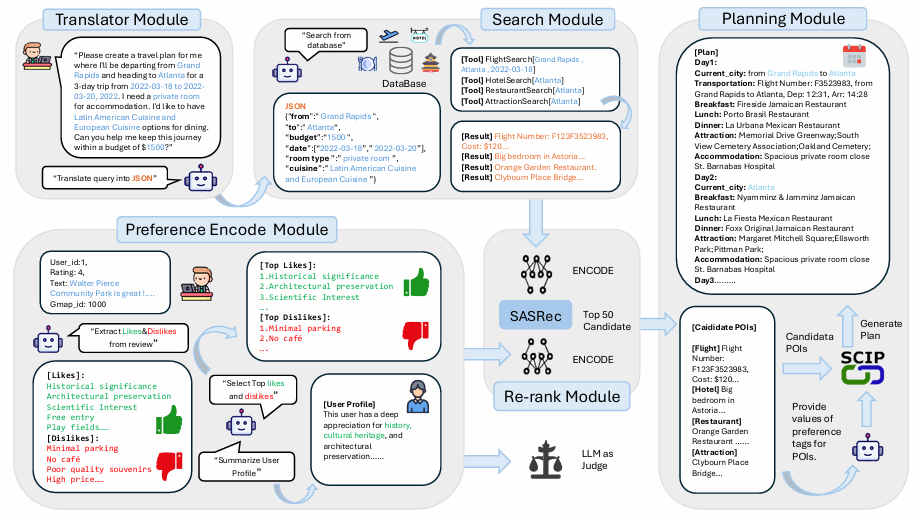
\includegraphics[width=0.7\textwidth]{images/image7.png}
\caption{แผนภาพสถาปัตยกรรมระบบ PTS (Personal Travel Solver Framework) (Shao et al., 2025)}
\end{figure}

จากภาพที่ 6 อธิบายองค์ประกอบและหน้าที่ของแผนภาพสถาปัตยกรรมระบบ PTS (Personal Travel Solver Framework)

\begin{enumerate}[leftmargin=1.5cm]
\item โมดูลการแปลความหมาย (Translator Module): ทำหน้าที่รับคำสั่งภาษาธรรมชาติจากผู้ใช้และใช้ LLM แปลงข้อมูลให้อยู่ในรูปแบบเชิงสัญลักษณ์ (Symbolic Representation) เช่น โครงสร้าง JSON เพื่อสกัดข้อจำกัดที่ชัดเจน (Explicit Constraints) ออกมาให้ระบบคอมพิวเตอร์เข้าใจได้
\item โมดูลการค้นหา (Search Module): นำเงื่อนไขที่ได้จากการแปลความหมายไปสืบค้นข้อมูลเบื้องต้น (Candidate Information) จากฐานข้อมูล เช่น ข้อมูลเที่ยวบิน โรงแรม และสถานที่ท่องเที่ยว (POIs) ที่สอดคล้องกับข้อจำกัดพื้นฐานของผู้ใช้
\item โมดูลเข้ารหัสความชอบ (Preference Encode Module): ใช้ LLM วิเคราะห์ประวัติการรีวิวหรือพฤติกรรมในอดีตของผู้ใช้ เพื่อสกัดสิ่งที่ชอบและไม่ชอบ จากนั้นแปลงค่าเป็น ``คะแนนความพึงพอใจ (Preference Score)'' สำหรับใช้เป็นเกณฑ์ในการเลือกสถานที่
\item โมดูลจัดอันดับใหม่ (Re-rank Module): นำรายการสถานที่และบริการจากโมดูลการค้นหา มาจัดเรียงลำดับใหม่โดยอิงจากคะแนนความพึงพอใจ เพื่อคัดกรองและดันตัวเลือกที่ตรงกับรสนิยมของผู้ใช้มากที่สุดขึ้นมาเป็นอันดับต้น ๆ
\item โมดูลการวางแผน (Planning Module): นำข้อมูลที่ผ่านการคัดกรองและจัดอันดับแล้วส่งเข้าสู่ตัวแก้ปัญหาทางคณิตศาสตร์ (Numerical Solver เช่น SCIP Solver) เพื่อคำนวณและจัดตารางเวลาที่สมบูรณ์แบบ โดยพิจารณาทั้งข้อจำกัดของผู้ใช้และข้อจำกัดเชิงสามัญสำนึก (เช่น เวลาเดินทาง การไม่ทับซ้อนกันของกิจกรรม)
\end{enumerate}

\subsection{งานวิจัยที่เกี่ยวข้อง}

การศึกษางานวิจัยที่เกี่ยวข้องถือเป็นขั้นตอนสำคัญสำหรับการสร้างกรอบแนวคิดในการพัฒนา Dino: The Central Application for Tourism in Khon Kaen ซึ่งมุ่งพัฒนาแพลตฟอร์มศูนย์กลางเพื่อสนับสนุนการท่องเที่ยวในจังหวัดขอนแก่น โดยรวบรวมข้อมูลแหล่งท่องเที่ยว ร้านอาหาร ที่พัก กิจกรรม และบริการต่าง ๆ พร้อมระบบวางแผนการเดินทางที่ใช้ปัญญาประดิษฐ์ (AI) เพื่อช่วยสร้างประสบการณ์การท่องเที่ยวที่เหมาะสมกับความต้องการของผู้ใช้งาน

เพื่อตอบโจทย์นี้ มีการทบทวนงานวิจัย 8 ชิ้น ที่เกี่ยวข้องกับ AI, Smart Tourism, Recommendation Systems, Chatbots, Sustainable Tourism, Traveler Engagement และ Microservices Architecture ซึ่งช่วยให้เห็นแนวโน้มหลักในการออกแบบระบบท่องเที่ยวอัจฉริยะ รวมถึงช่องว่างขององค์ความรู้ (Research Gaps) และแนวทางการต่อยอด (Implications) ที่ Dino สามารถพัฒนาได้

\subsubsection{การใช้ AI เพื่อพัฒนาระบบแนะนำการท่องเที่ยวและ Trip Planning}

งานของ Banerjee et al. (2025) นำเสนอการใช้ Retrieval-Augmented Generation (RAG) เพื่อพัฒนาระบบแนะนำการท่องเที่ยวแบบยั่งยืน โดยระบบจะดึงข้อมูลจากหลายแหล่ง เช่น บทความรีวิว สถิติการท่องเที่ยว และโซเชียลมีเดีย จากนั้นสร้างคำแนะนำที่เหมาะสมกับความสนใจเฉพาะบุคคลมากขึ้น ซึ่งช่วยปรับปรุงคุณภาพของคำแนะนำให้ตรงกับโปรไฟล์ของผู้ใช้งาน (Banerjee et al., 2025)

ผลการศึกษานี้สอดคล้องกับงานของ Jyothi et al. (2025) ที่พัฒนา Travel Finder ซึ่งใช้ Collaborative Filtering และ Clustering Algorithms เพื่อสร้างกลุ่มนักท่องเที่ยวตามความสนใจและลักษณะการเดินทาง ผลการทดลองพบว่าระบบสามารถลดเวลาในการค้นหาแหล่งท่องเที่ยวลง 34\% และเพิ่มความพึงพอใจของผู้ใช้งานได้อย่างมีนัยสำคัญ ซึ่งสนับสนุนข้อค้นพบของ Banerjee et al. (2025) ว่าการใช้ AI เพื่อปรับคำแนะนำให้ตรงกับความต้องการส่วนบุคคล (Personalization) เป็นปัจจัยสำคัญต่อประสบการณ์ของนักท่องเที่ยว

อย่างไรก็ตาม ทั้งสองงานมีความแตกต่างกันในด้านแนวทาง Banerjee et al. (2025) มุ่งเน้นการสร้างระบบแนะนำเชิงข้อมูลเชิงลึก (Data-driven Recommendations) ผ่านการใช้โมเดลภาษาขนาดใหญ่ (LLMs) ขณะที่ Travel Finder ของ Jyothi et al. (2025) มุ่งเน้นการจับกลุ่มผู้ใช้ตามพฤติกรรมจริงเพื่อต่อยอดการแนะนำแบบ Social-based Recommendation ความแตกต่างนี้เปิดโอกาสให้ Dino สามารถผสมผสานข้อดีของทั้งสองวิธีเพื่อสร้างระบบที่ทั้ง แม่นยำ และ ยืดหยุ่น ในการแนะนำเส้นทางและกิจกรรมการท่องเที่ยว

\subsubsection{AI และ Chatbot เพื่อยกระดับประสบการณ์ผู้ใช้}

(University College of Goizha et al., 2023) พัฒนาระบบ Chatbot Tourist Guide โดยใช้ Artificial Intelligence Markup Language (AIML) เพื่อสร้างการสนทนาที่เป็นธรรมชาติกับนักท่องเที่ยว ระบบนี้สามารถตอบคำถามพื้นฐาน เช่น สถานที่ท่องเที่ยว ร้านอาหาร และข้อมูลตั๋วเข้าชม ผลการทดลองกับนักท่องเที่ยว 150 คน พบว่า 78\% ของผู้ใช้พึงพอใจกับความเร็วและความถูกต้องของคำตอบ นอกจากนี้ Chatbot ยังช่วยลดภาระงานของเจ้าหน้าที่ศูนย์บริการนักท่องเที่ยวลงถึง 40\%

ผลนี้สอดคล้องกับงานของ Deshmukh et al. (2025) ที่พัฒนาแพลตฟอร์ม AI-powered Personalized Itinerary Planning ซึ่งมี Chatbot ทำงานร่วมกับ Recommendation Engine เพื่อสร้างแผนการท่องเที่ยวอัตโนมัติ โดย Chatbot สามารถดึงข้อมูลแบบเรียลไทม์ เช่น สภาพอากาศ การจราจร และราคาที่พัก เพื่อปรับคำแนะนำให้สอดคล้องกับสถานการณ์ปัจจุบัน ผลการทดสอบกับกลุ่มนักท่องเที่ยว 300 คน พบว่า 85\% ของผู้ใช้ยืนยันว่าแผนการเดินทางที่ระบบสร้างให้มีความเหมาะสมและตรงตามความต้องการสูง

จากการสังเคราะห์ พบว่าทั้งสองงานสนับสนุนข้อสรุปสำคัญว่า Chatbot ไม่ได้เป็นเพียงเครื่องมืออำนวยความสะดวก แต่สามารถทำหน้าที่เป็น ตัวกลางในการวิเคราะห์ข้อมูลแบบเรียลไทม์ ซึ่งช่วยปรับแผนการท่องเที่ยวให้เหมาะสมมากขึ้น อย่างไรก็ตาม ความแตกต่างระหว่าง AIML-based Chatbot ของ University College of Goizha et al. (2023) และระบบ AI-integrated Chatbot ของ Deshmukh et al. (2025) แสดงให้เห็นโอกาสในการพัฒนา Dino ให้รองรับ Natural Language Processing (NLP) ที่มีความฉลาดและยืดหยุ่นมากยิ่งขึ้น

\subsubsection{การจัดการข้อมูล การวิเคราะห์พฤติกรรม และการมีส่วนร่วมของนักท่องเที่ยว}

Ma et al. (2025) ศึกษาการใช้ AI เพื่อเพิ่มการมีส่วนร่วมของนักท่องเที่ยว (Traveler Engagement) และการจัดการจุดหมายปลายทาง (Destination Management) โดยใช้เทคนิค Heatmap Analytics และ Real-time Behavioral Tracking เพื่อระบุพื้นที่ที่นักท่องเที่ยวให้ความสนใจสูง ผลการทดลองแสดงให้เห็นว่าข้อมูลเชิงพฤติกรรมช่วยให้หน่วยงานท้องถิ่นปรับปรุงการจัดสรรทรัพยากรและออกแบบแผนการตลาดที่ตอบโจทย์ได้มากขึ้น

\begin{figure}[h]
\centering
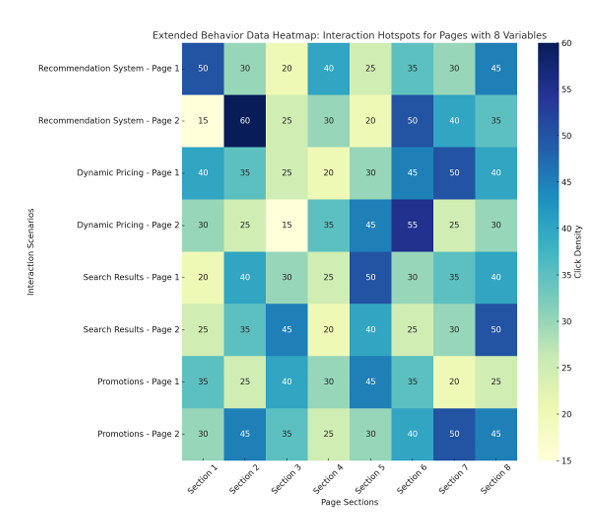
\includegraphics[width=0.7\textwidth]{images/image8.png}
\caption{แผนภาพ Heatmap แสดงข้อมูลเชิงพฤติกรรม (Ma et al., 2025)}
\end{figure}

การวิเคราะห์ Heatmap ของข้อมูลพฤติกรรมผู้ใช้จากสามแพลตฟอร์มท่องเที่ยวออนไลน์แสดงในภาพที่ 7 Heatmap นี้สื่อถึงการกระจาย ``ความเข้มข้นของการปฏิสัมพันธ์'' ของผู้ใช้ในส่วนต่าง ๆ ได้แก่ ระบบแนะนำ การกำหนดราคาแบบไดนามิก ผลการค้นหา และหน้าโปรโมชัน ด้วยการไล่ระดับสีจากเหลืองอ่อน (ความเข้มต่ำ เช่น ค่าถ่วงน้ำหนัก 15) ไปจนถึงน้ำเงินเข้ม (ความเข้มสูง เช่น 60) แกนแนวนอนแบ่งเป็น 8 ส่วนของหน้า (Section 1--8) ส่วนแกนแนวตั้งเป็นฮอตสปอตการปฏิสัมพันธ์ในฉากการใช้งานของหน้าประเภทต่าง ๆ

ภาพรวม บทบาทของปัญญาประดิษฐ์ (AI) ช่วยยกระดับประสบการณ์ผู้ใช้และประสิทธิภาพการตัดสินใจ ทั้งในระบบแนะนำแบบปรับให้เหมาะกับบุคคล (personalized recommendations) การกำหนดราคาแบบไดนามิก และการปรับแต่งผลการค้นหา อย่างไรก็ดี ยังมีประเด็นที่ควรปรับปรุงเพื่อเพิ่มความเชื่อมั่นและคุณภาพประสบการณ์

ขณะเดียวกัน Sousa et al. (2024) ทำการสำรวจความคิดเห็นนักท่องเที่ยวจำนวน 500 คน เกี่ยวกับการใช้ AI ในการวางแผนการเดินทางและการเข้าถึงข้อมูล ผลการศึกษาพบว่า 72\% ของนักท่องเที่ยวเลือกใช้แพลตฟอร์มที่มี AI ในการแนะนำสถานที่ท่องเที่ยว และ 68\% ยืนยันว่าพวกเขามีแนวโน้มที่จะกลับมาใช้บริการซ้ำ หากระบบสามารถปรับคำแนะนำให้เหมาะกับพฤติกรรมการท่องเที่ยวส่วนบุคคล

การเปรียบเทียบสองงานนี้พบว่าทั้ง Ma et al. (2025) และ Sousa et al. (2024) ชี้ให้เห็นถึงความสำคัญของ Data-driven Personalization และ Traveler Engagement แต่ต่างกันที่ Ma et al. (2025) มุ่งเน้นการวิเคราะห์เชิงเทคนิคเพื่อช่วยองค์กรปรับปรุงโครงสร้างการจัดการ ขณะที่ Sousa et al. (2024) มุ่งสำรวจพฤติกรรมและความต้องการของผู้บริโภคโดยตรง ซึ่งแสดงให้เห็นว่าการพัฒนา Dino ควรผสมผสานข้อมูลทั้งสองฝั่งเข้าด้วยกันเพื่อให้เกิดแพลตฟอร์มที่ ตอบโจทย์ทั้งนักท่องเที่ยวและผู้กำหนดนโยบาย

\subsubsection{LLM as a Judge}

\subsubsection{บทวิเคราะห์แนวโน้มและช่องว่างการวิจัย}

จากการวิเคราะห์งานวิจัยทั้ง 8 ชิ้น พบว่าแนวโน้มหลักของการวิจัยด้าน AI ในการท่องเที่ยว มุ่งเน้นไปที่การสร้างประสบการณ์การท่องเที่ยวที่เป็นส่วนบุคคลมากขึ้น และการพัฒนาระบบสนับสนุนการตัดสินใจของผู้ใช้ งานของ Banerjee et al. (2025) นำเสนอการใช้ Retrieval-Augmented Generation (RAG) เพื่อพัฒนาระบบแนะนำสถานที่ท่องเที่ยวที่มีความแม่นยำสูง ขณะที่ Deshmukh et al. (2025) มุ่งเน้นการสร้างแผนการเดินทางที่ปรับเปลี่ยนตามข้อมูลเรียลไทม์ เช่น สภาพอากาศและความหนาแน่นของนักท่องเที่ยว สำหรับงานของ Jyothi et al. (2025) นำเสนอ Travel Finder ที่ใช้ Collaborative Filtering และ Clustering เพื่อสร้างระบบแนะนำที่ตอบสนองต่อความสนใจของผู้ใช้ ส่วน University College of Goizha et al. (2023) พัฒนา Chatbot เพื่อให้ข้อมูลและโต้ตอบนักท่องเที่ยวแบบอัตโนมัติ ซึ่งสอดคล้องกับ Ma et al. (2025) ที่มุ่งเน้นการวิเคราะห์พฤติกรรมและเพิ่มการมีส่วนร่วมของนักท่องเที่ยวผ่านเทคนิคการวิเคราะห์ข้อมูลเชิงลึกแบบเรียลไทม์

อย่างไรก็ตาม เมื่อสังเคราะห์เนื้อหาของงานวิจัยพบว่า ช่องว่างองค์ความรู้ที่สำคัญยังคงอยู่ในประเด็น การบูรณาการข้อมูลหลายระบบเข้าด้วยกัน ในขณะที่การวางแผนการเดินทางมีความแม่นยำและเป็นส่วนตัวมากขึ้นผ่านการผสาน LLM เข้ากับ Numerical Solvers เพื่อจัดการข้อจำกัดที่ซับซ้อนตามที่ Shao et al. (2025) นำเสนอ และรองรับการขยายตัวด้วยสถาปัตยกรรมไมโครเซอร์วิสของ Barua \& Kaiser (2024) แต่ยังไม่เชื่อมโยงกับฐานข้อมูลของภาครัฐหรือข้อมูลเชิงนโยบาย ในขณะเดียวกัน Sousa et al. (2024) และ Milton \& Philosophers (2023) ชี้ให้เห็นถึงความท้าทายด้าน ความเป็นส่วนตัวของข้อมูลและธรรมาภิบาล ซึ่งยังไม่ได้รับการแก้ไขอย่างสมบูรณ์ สรุปได้ว่าปัจจุบันแม้ AI จะเข้ามามีบทบาทสำคัญในภาคการท่องเที่ยว แต่ยังขาด แพลตฟอร์มแบบบูรณาการ ที่เชื่อมโยงข้อมูลหลายมิติ เพื่อรองรับการพัฒนาเชิงพื้นที่และสร้างการท่องเที่ยวที่ยั่งยืน
